\documentclass{strrespaper-trad}
\usepackage[utf8]{inputenc}
\usepackage[T1]{fontenc}
\usepackage{csquotes}
\usepackage[english]{babel}

% For math
\usepackage{amsmath}

% For better tables
\usepackage{booktabs}
\usepackage{threeparttable}

% For images
\usepackage{graphicx}

% For subfigures
\usepackage{subfig}

% For landscape pages
\usepackage{pdflscape}

% For drawing
\usepackage{tikz}
\usetikzlibrary{shapes.multipart}

% For plotting
\usepackage{xcolor}
\usepackage{pgfplots}
\pgfplotsset{compat=1.16}

% For units
\usepackage{siunitx}
\sisetup{
	separate-uncertainty=true
}

% For Project Plan
\usepackage{pgfgantt}
\usepackage{tabularx}

% For code listings (type "texdoc listings" [without the quotes] for more information)
% \usepackage{listings}

\newcommand{\mnk}{\textit{m, n, k} game}
\newcommand{\mnkpl}{\textit{m, n, k} games}
\newcommand{\ttt}{Tic-Tac-Toe}
\newcommand{\TTT}{TIC-TAC-TOE}

% Required for the citations
\usepackage[style=apa,sortcites=true,sorting=nyt,backend=biber]{biblatex}
\addbibresource{../str-templates/sample-resources/bibliographies/str.bib} % TODO: Remove
\addbibresource{../paleo-str-g12.bib}

 
\title{Comparison of Genetic Algorithm Training Methods As Applied To \ttt}

\usepackage[calc]{datetime2}
\makeatletter
\newcommand{\daymonthyear}{\@dtm@day\ \DTMenglishmonthname{\@dtm@month} \@dtm@year}
\makeatother
\date{\daymonthyear}

\tptitle{
	Comparison Of Genetic Algorithm Training Methods\\
	As Applied To \TTT
}
\addAuthor{Vash Patrick B. Ancheta}
\addAuthor{Diego Sulayman R. Pascua}
\addAuthor{Resh Vnzi S. Togue\~no}
\adviser{Kaye Melina Natividad B. Alamag}
\level{3}

\begin{document}
	\maketitle

	\frontmatter

	\unnumchapter*{APPROVAL SHEET}
		\makeapprovalsheet{
			\signatureline{Conrado C. Rotor, \NoCaseChange{Jr., Ph.D.}}{Chair}

			\signatureline{Melba C. Patacsil}{Co-chair}

			\vspace*{\baselineskip}

			\begin{multicols}{2}
				\begin{center}
					\signatureline{Jay Jay F. Manuel}{Member}
					\signatureline{Ricarido M. Saturay, \NoCaseChange{Jr.}}{Member}

					\columnbreak

					\signatureline{Marites P. Rivera}{Member}
					\signatureline{Freda M. Wong}{Member}
				\end{center}
			\end{multicols}
		}

	\unnumchapter*{ACKNOWLEDGEMENT}
		We are grateful for our friends and family for their continued support in our continuous lives.
		We are also thankful to our teachers, research teacher, and research adviser for their unwavering assistance in having the research completed.
		Without these people, this research would never be successful.

	\unnumchapter{ABSTRACT}
		% TODO: Abstract
		% Do note that abstracts should not contain references.
		\makeabstract{
			According to \textcite{georgemasonuniversityWritingAbstract2020}, \blockquote{An abstract is a 150- to 250-word paragraph that provides readers with a quick overview of your essay or report and its organization. It should express your thesis (or central idea) and your key points; it should also suggest any implications or applications of the research you discuss in the paper.}
			\textcite{georgemasonuniversityWritingAbstract2020} also states that the common abstract is divided into such: 25\% of space on the purpose and importance of the research (Introduction), 25\% of space on what was done (Methods), 35\% of space on what was found (Results), and 15\% of space on the implications of the research.
		}

	\unnumchapter*{Table of Contents}
		\contents
		% \listoflistings

	\mainmatter

	\chapter{INTRODUCTION}
		\section{Background of the Study}
			% TODO: Background of the Study
			Machine learning (ML) is vast---it is used in different situations such as spam detectors, web search engines, photo tagging applications and game development \autocite{sharmaMachineLearningApplications2016}.
			There have been researches that are aimed at improving the implementation of ML in various games.
			A category of games under investigation through ML is the set of \mnk\ games, comprised of games where there is an $m \times n$ grid and two players alternate turns trying to earn $k$ pieces adjacent to each other horizontally, vertically or diagonally \autocite{hayesDevelopingMemoryEfficient2016}.
			Among the most common examples of \mnkpl\ are G\=o, Othello, and Chess.
			\ttt, the game under investigation in this study, is an example of an \mnk.
			A \ttt\ board is composed of three rows and three columns, and requires three adjacent pieces of the same player to render a win, thus it is considered to have a $3, 3, 3$ configuration.

			Improvements in ML have lead to the development of artificial intelligence (AI) players that can beat even the most competitive human players around the world.
			Machine learning methods (MLMs) are algorithms where machines are not explicitly programmed to do what is tasked.
			Rather, similar to its namesake, MLM-trained machines are capable of performing tasks given its own internal code without any human interference.
			In short, the machine \textit{learns} \autocite{geeksforgeeksMachineLearning}.
			An example of an MLM is the genetic algorithm (GA).

			This study aims to develop multiple GAs with different elite preservation methods and compare their performance in \ttt\ based on the possible situations.

		\section{Objectives of the Study}
			\subsection{General Objective}
				\begin{itemize}
					\item To compare the effectiveness of trained genetic algorithm (GA) organisms among each other as applied to \ttt
				\end{itemize}
			\subsection{Specific Objectives}
				\begin{enumerate}
					\item To implement known heuristics into Python code
					\item To train organisms of an implemented GA using different move generators (MGs)
					\item To compare the development of the performance of trained GA organisms among each other within 500 generations
				\end{enumerate}

		\section{Significance of the Study}
			% TODO: Significance of the Study
			This study will contribute to the body of knowledge in ML.
			Through this study, more can be known about how information gained from one method of AI can be passed on to another mechanism of AI through training.
			This will shed light on how information from one AI player can be transmitted to an MLM such as GA.
			This, by extension, can improve the comprehension of how machines can learn strategies in games from one with greater skill.

		\section{Scope and Limitations of the Study}
			% TODO: Scope and Limitations of the Study
			This study will focus only on \ttt\ and not other games such as Chess or G\=o because it is the simplest game to conduct the research on heuristics, namely the training of the GA under different MGs.
			The complexity of the board game is not relevant to the study because the focus of the research is to compare the effectiveness of trained GA organisms given an \mnk.
			Applying these heuristics on other \mnkpl\ however are beyond the time frame of the research.
			The study will only develop three GAs.
			The first is a Python implementation of the GA in the work of \textcite{bhattSearchNolossStrategies2008}.
			Using developed AI, the second and third are modified implementations of the same GA.
			The performance of each GA will be based on how many generations it will take for the GA to find a no-loss first player for \ttt.
			This basis for comparison of performance, specifically using the skill of an organism as a first player, is due to the fact that Python is known for being slow.
			In line with this, indices are 0-based in this paper, as they are in Python.

	\unnumchapter{DEFINITION OF TERMS}
		% TODO: Definition of Terms
		\termdef{\mnk}{
			a game where there is an $m \times n$ grid where two players alternate turns trying to earn $k$ pieces adjacent to each other horizontally, vertically or diagonally
		}
		\termdef{Artificial Intelligence (AI)}{
			program that simulates human actions, can simulate a human player in a game.
		}
		\termdef{Allele}{
			the configuration value of a gene given a unique organism
		}
		\termdef{Genetic Algorithm (GA)}{
			algorithm that simulates natural selection and biological reproduction to produce solutions to a problem
		}
		\termdef{Gene}{
			representation of a unique and distinct situation in a game given the game rules
		}
		\termdef{Genome}{
			mapping table of genes with corresponding alleles
		}
		\termdef{Machine Learning (ML)}{
			a heuristic where a program learns rather than strictly follow a given instruction
		}
		\termdef{Machine Learning (MLM)}{
			algorithms used in machine learning
		}
		\termdef{Organism}{
			an algorithm represented by a genome
		}
		\termdef{Probability Valuation (PV)}{
			classical probability of a player winning at a given game state
		}
		\termdef{\ttt}{
			\mnk\ configured as 3,3,3
		}

	\chapter{REVIEW OF RELATED LITERATURE}
		% TODO: Review of Related Literature
		\section*{Effective Computer Algorithms on \ttt}
			There have already been precedents in investigating the proper method of winning classic \ttt.
			Examples such as prioritizing the center or placement of pieces in the opposite cell of the opponent's previous move are frequently cited as techniques to beat the opponent \autocite{aycockHowWinTicTacToe2002}.
			Multiple discussions gave occurred on how many distinct games one can play in \ttt.
			\textcite{schaeferHowManyGames2002} argues that the common answer of 9! or 362,880 possible games is misleading for it ignores the symmetrical properties of the game.
			There are games that have exactly the same pieces placed on the board but are oriented differently in relation to the board.
			For example, a gametree turned 90\textdegree\ is considered a distinct game state in the 9! calculation.
			According to \textcite{schaeferHowManyGames2002}, it is of more concern to count game states that end when there are $k$ adjacent pieces.
			Using this method of counting game states, \textcite{schaeferHowManyGames2002} computed a total number of 765 distinct game states.

			Numerous studies have been performed on the most effective algorithms for a computer program to win in \ttt.
			In organizing the results of a computer algorithm, one of the most common methods of organization is the use of a game tree.
			A game tree is a collection of all possible game states arranged in chronological order.
			The root node represents the current state, its child node the set possible game states.
			The edges represent the moves and the terminal nodes represent game states that indicate a completed game.
			The game tree begins from the root node and branches out into nodes that have their own children \autocite{adamchikGameTrees2009}.
			A diverse game tree is optimal for exploring the capabilities of the different machine learning methods to be used in the study.

			\begin{figure}
				\centering
				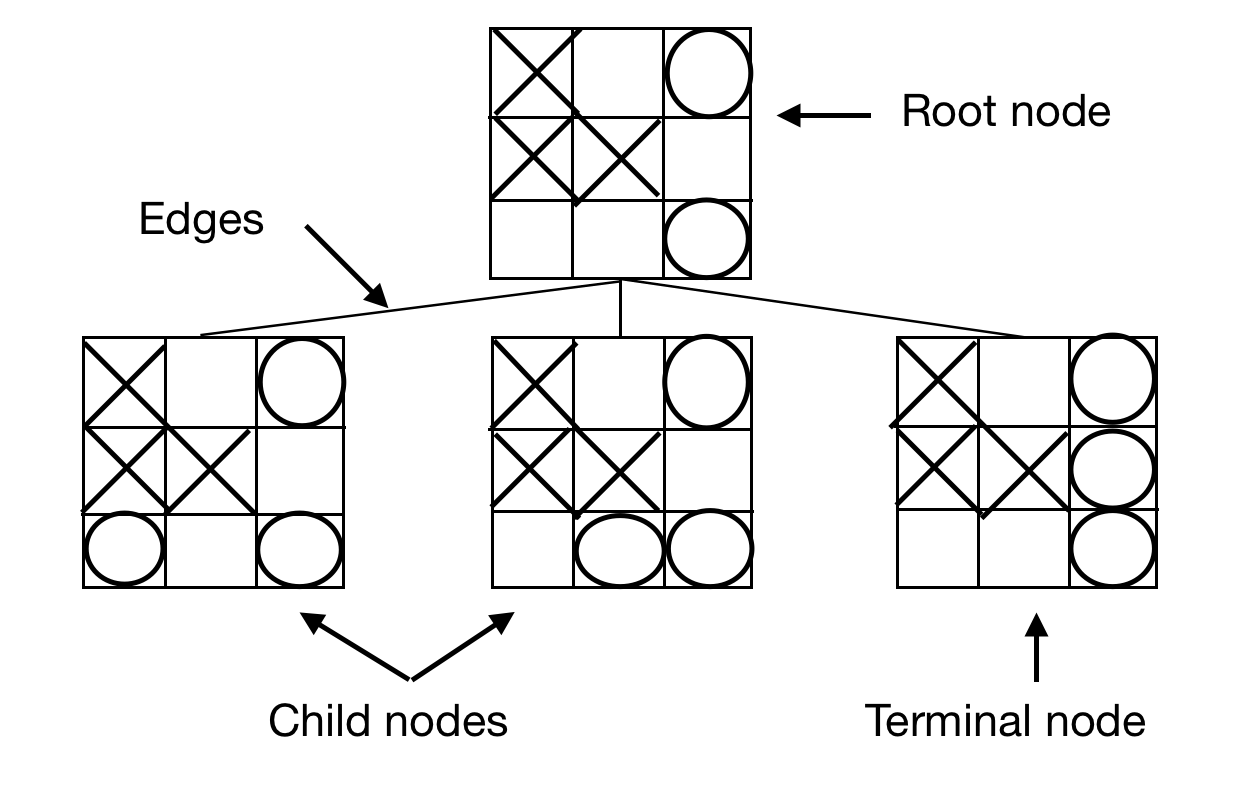
\includegraphics[width=0.7\linewidth]{gametree}
				\caption{Game tree}
				\label{fig:gametree}
			\end{figure}

			A study by \textcite{cranenburghTicTacToe2007} is concerned with the use and implementation of a heuristic known as depth-first search. Depth-first search is a machine learning method that utilizes \textit{backtracking}.
			When the algorithm encounters a terminal node, it returns to the previous nodes to find other possible nodes, hence the term \textit{backtracking} \autocite{hackerearthDepthFirstSearch2019}.
			According to \textcite{cranenburghTicTacToe2007}, a higher depth search with more game states, leads to a higher win rate or at least, leads the program to reach a draw better.

			Researches that deal with the more complex \ttt\ variant Ultimate/Super \ttt\ seek to find the patterns and implementing these patterns into AI.
			Analogous to how classic \ttt\ is symmetric, a study by \textcite{georgeGroupActionsWinning2016} specifies the rotational and reflectional symmetry of Ultimate/Super \ttt.
			A study by \textcite{lifshitzAIApproachesUltimate} deals with the use of a mixture of heuristics and algorithms such as MiniMax (an algorithm that traverses the whole game tree) and ExpectiMax (an algorithm that analyzes the expectations of the opponent's moves).
			Given a controlled set of parameters, ExpectiMax won against a random algorithm most of the time.
			When played against MiniMax however, ExpectiMax was more likely to lose.
			This is in agreement with the aforementioned conclusion that an increased depth produces better results.
			A caveat for this machine learning method is the drastic duration of time the algorithm requires with each increase in depth.
			The higher the depth of the depth-first search, the longer the time needed for the algorithm to provide the most optimal move.

		\section*{Machine Learning Methods}
			Various methods of machine learning have been discovered prior.
			One of the earliest examples of machine learning methods is Hexapawn formulated by Martin Gardner.
			The game is composed of a $3 \times 3$ board with two sets of three pawns in a row on opposite sides of the board, and the players move alternately.
			The game is typically played by a human (who always goes first) and an AI player.
			A player wins the game by accomplishing one of three goals: move a pawn to the opposite edge, capture all enemy pieces, or leave the enemy with no moves.
			Because of the small scale of the game and its symmetry, all the possible game states can be represented in 24 cards.
			Each of these cards contains a move performed by the human player and arrows of different colors representing the possible moves the AI player can take \autocite{ortizMachineLearningHexapawn2017}.
			The AI player contains a matchbox for each card representing a game state.
			These matchboxes contain beads that correspond to the possible moves the AI player may make.
			During play, the beads are chosen at random and the AI player moves according to the bead taken.
			If the move made by the AI player leads to the loss of the AI, the bead corresponding to the move is taken away.
			Otherwise, the bead is returned to the matchbox.
			After 50 games, the AI player is practically unbeatable as game states with high probability of loss is reduced \autocite{gardnerMathematicalGames1958}.

		\section*{Genetic Algorithm}
			Living organisms exhibit a level of problems solving that is almost impossible to be recreated by a computer scientist.
			Even more, the complexity that living organisms show is one that is incredibly enviable to a computer scientist wanting to achieve some problem solving program; problems that computer scientists have spent endless amounts of intellectual effort on have been solved by living organism without any thought, relying on the process of evolution.

			Due to this, many researchers have began emulating the process of evolution on their algorithms, subjecting their own programs to a process of reproduction and natural selection.
			This method is widely used in the realm of machine learning, since it eliminates a great hurdle in software engineering: programmers need not to specify the individual aspects of each program and the means that actions are carried out.

			\begin{figure}
				\centering
				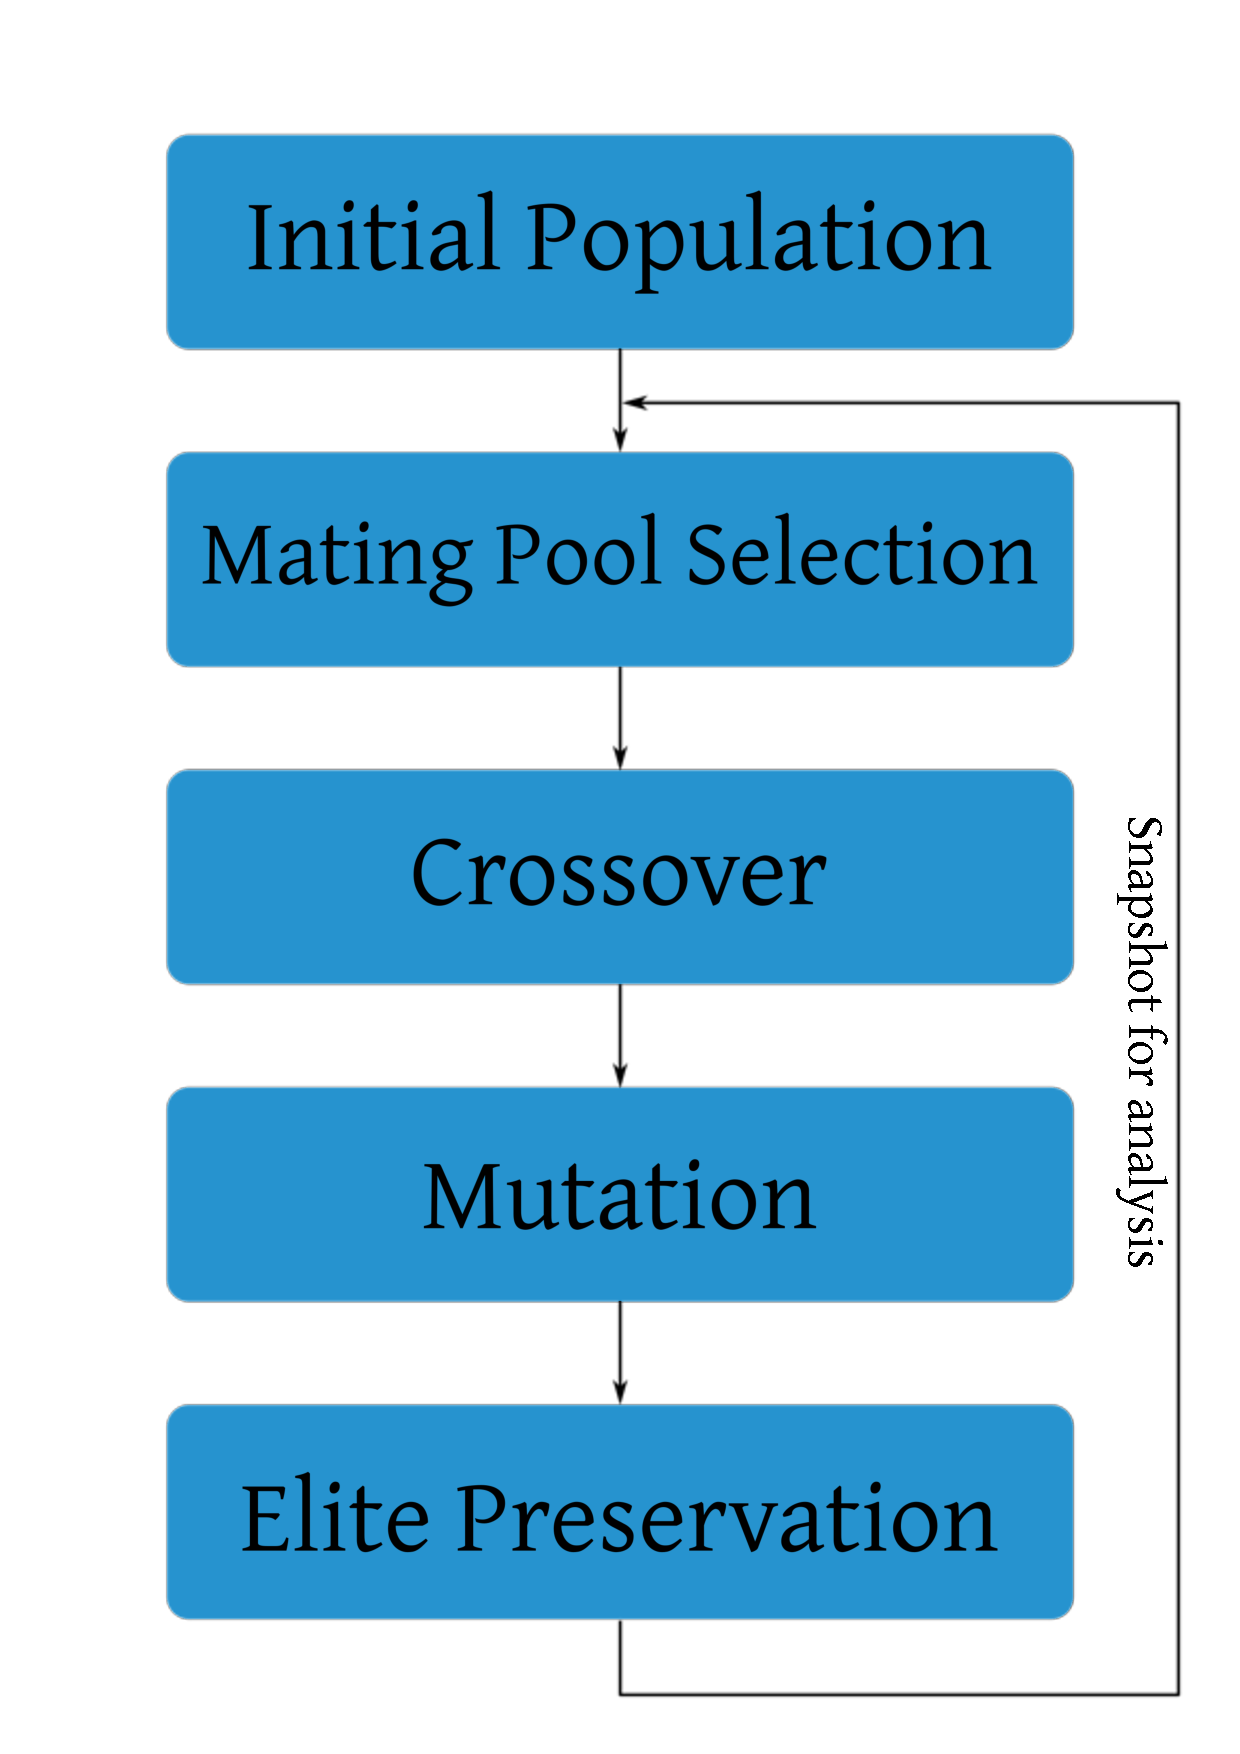
\includegraphics[width=0.6\linewidth]{genetic}
				\caption{Flowchart of GA training}
				\label{fig:genetic}
			\end{figure}

			There are two aspects of the evolution process that computer scientists want to emulate: natural selection and reproduction. "Natural selection" is the process of choosing which solutions survive to make a new generation of algorithms, the survivors govern the characteristics of next generation. Reproduction is the recombination of genes from parent to offspring, making the "child" algorithm of an organism have similar characteristics to their two parent algorithms.

			Programming natural selection is done by giving an algorithm a test of fitness, going through numerous iterations, then giving a fitness score based on that performance \autocite{hochmuthGeneticEvolutionPerfect2003}.
			Fitness scores are usually calculated based on the ratio of games won, as shown in Equation~\ref{eqn:fitness}.
			The higher the fitness score, the higher the changes of winning with the solution or the move done in the game.
			Algorithms with low fitness scores are discarded and those with high fitness scores move on to reproduction.
			\begin{equation}
				f(x_i) = \frac{n_\mathrm{lost}}{n_\mathrm{games}} \label{eqn:fitness}
			\end{equation}
			The emulation of reproduction is far more complicated.
			Originally, it was based on random mutation of the algorithms, however this oftentimes produces algorithms that would not run, or are drastically different from the intended purpose of the program.
			Later development focuses on adding together characteristics from the two parents.
			This was also limited since this could only be done to characteristics that could be added meaningfully \autocite{hollandGeneticAlgorithms}.

			Currently, reproduction is done by means of a classifier system.
			A classifier system is a system where conditions and actions are represented by strings of ones and zeroes corresponding to the presence or absence of that characteristic.
			For example, as shown in Table \ref{tab:ex_classifier}, since humans have eyes and opposable thumbs and require oxygen, but do not have wings or gills, humans can be recorded as [10011], while the only recorded characteristic of the bacterium that is present is that it requires oxygen, so it is recorded as [00001].
			Reproduction can now be done on these "genes" by recombining different genes and making new offspring.
			In the computer science world, these aspects are usually very basic and primitive, but with strings with lengths reaching tens of thousands of bits long.

			\begin{table}[htbp]
				\centering
				\begin{tabular}{lccc}
					\toprule
					Aspect           & Human & Fish & Bacterium \\
					\midrule
					opposable thumbs & 1     & 0    & 0         \\
					wings            & 0     & 0    & 0         \\
					gills            & 0     & 1    & 0         \\
					eyes             & 1     & 1    & 0         \\
					requires oxygen  & 1     & 1    & 1         \\
					\bottomrule
				\end{tabular}
				\caption{Example of Organisms Sorted Through a Classifier System}
				\label{tab:ex_classifier}
			\end{table}

	\chapter{MATERIALS AND METHODS}
		\section{Research Design}
			This Developmental Research is composed of two components: Software Development and Data Collection.
			In Software Development the code for the move generators and genetic algorithms are initialized, and the efficiency of its implementation is optimized.
			In Data Collection the organisms will be trained for 500 generations, and the fitness data collected will be analyzed using $R$.
			The independent variable is the elite preservation method.
			The dependent variable is the number of generations the specific GA takes to find a no-loss solution.
			Extraneous variables such as the software specifications can be held constant by the use of the same software such as the operating system and the same Python version (3.8.3 64-bit).
			The study will not be affected by hardware specifications as it concerns the number of generations instead of the time taken on the system.

		\section{Locale of the Study}
			The software will be developed and data will be collected mainly at the Philippine Science High School -- Cordillera Administrative Region Campus.
			The training and data collection will proceed at the aforementioned location on various personal computers.

		\section{Materials and Research Instruments}
			The software will be developed with Python 3.8.3 on KDE Neon 5.18 using Visual Studio Code 1.45.1 and hosted on GitHub.
			A link to the repository hosting the software is located in \ref{apx:documentation}.
			The developmental computer is equipped with 4 GB of Random Access Memory (RAM).
			Various personal computers will be used to perform the training.

		\section{Procedures}
			% TODO: Procedures
			An elaborate and chronological description of the procedures to be taken is provided in this section.
			The proper reasoning for each step taken should be stated, as well as what materials and research instruments are used in each step.

		\section{Treatment of Data}
			\subsection{Statement of Hypotheses} \vspace{-2em}
				\begin{align*}
					H_0 & : \mu_\mathrm{UMG} = \mu_\mathrm{fitness} = \mu_\mathrm{RMG} \\
					H_a & : \text{The means are not all equal}
				\end{align*}
			\subsection{Analysis of Data}
				The data will be analyzed through the $R$ with the use of Analysis of Variance (ANOVA) which gives the $p$-value to test the hypotheses at a given confidence interval.
				The study will utilize $\alpha = 0.10$.
				Should the alternative hypothesis be true, Tukey Honest Significant Differences (Tukey HSD) will be applied to locate the different mean.

	\chapter{RESULTS AND DISCUSSION}
		% TODO: Results and Discussion
		\textquote[\cite{skillsyouneed.comDissertationWritingResults2020}]{The Results section should set out your key experimental results, including any statistical analysis and whether or not the results of these are significant}.

		Cite literature that support your analyses of the results.
		It is imperative to include relevant results, regardless of support of hypotheses.
		Brief descriptions of the results should be provided when clarification is needed.

		\section*{Softening Points}
			\begin{figure}[ht]
				\centering
				\definecolor{grrayt}{HTML}{848484}
				\begin{tikzpicture}
					\begin{axis}[
							width  = \linewidth,
							height = 8cm,
							major x tick style = transparent,
							ybar=2*\pgflinewidth,
							bar width=\linewidth/12,
							ymajorgrids = true,
							ylabel = {Softening point (\si{\celsius})},
							symbolic x coords={0\% PP, 2\% PP, 4\% PP, 6\% PP},
							xtick = data,
							scaled y ticks = false,
							try min ticks = 10,
							enlarge x limits=0.25,
							ymin=0, ymax = 100
						]
						\addplot[style={grrayt,fill=grrayt,mark=none}, error bars/.cd,
							y dir=both, y explicit, error bar style={color=black}]
						coordinates {(0\% PP, 48.5)+-(4.0, 4.0) (2\% PP, 56.0)+-(2.0, 2.0) (4\% PP, 61.5)+-(2.5, 2.5) (6\% PP, 68.0)+-(2.0, 2.0)}
						node[pos=0/4,anchor=south, color=black, yshift=10] {48.5}
						node[pos=1/4,anchor=south, color=black, yshift=10] {56.0}
						node[pos=3/4,anchor=south, color=black, yshift=10] {61.5}
						node[pos=4/4,anchor=south, color=black, yshift=10] {68.0};
					\end{axis}
				\end{tikzpicture}
				\caption[Sample bar graph]{Sample bar graph of softening points}
				\label{fig:samplebargraph}
			\end{figure}

			\clearpage

			\begin{table}[htbp]
				\centering
				\begin{threeparttable}
					\caption[Characteristics of the Sample]{Characteristics of the Sample\tnote{\textdagger}}
					\label{tab:sample_characteristics}
					\begin{tabular}{llll}
						\toprule
						Variable                                     & Control         & Heat \& moisture exchanger & Probability \\
						                                             & (n = 45)        & (n = 49)                   &             \\
						\midrule
						Age (years)\tnote{1}                         & \num{32.7(35)}  & \num{36.3(27)}             & 0.08        \\
						Height (\si{\meter})\tnote{1}                & \num{1.72(60)}  & \num{1.67(80)}             & NS          \\
						Weight (\si{\kilo\gram})\tnote{1}            & \num{76.6(128)} & \num{72.3(162)}            & NS          \\
						Gender (number of males)\tnote{2}            & 21              & 26                         & NS          \\
						ASA Physical Status\tnote{3}                 & \num{2(1)}      & \num{2(1)}                 & NS          \\
						OR room temperature (\si{\celsius})\tnote{1} & \num{21.1(36)}  & \num{20.6(29)}             & NS          \\
						\bottomrule
					\end{tabular}
					\begin{tablenotes}
						\small
						\item[1]
						Data is expressed as mean \textpm{} one standard deviation.
						Probability determined using a two-tailed, unpaired Student's t-test.
						\item[2]
						Data is expressed as number within the sample who possess the characteristic.
						Probability determined using Chi square (or Fisher's Exact test for $2 \times 2$ tables).
						\item[3]
						Data is expressed as median \textpm{} one interquartile range.
						Probability determined using a Mann-Whitney U test.
						\item[\textdagger] Source: \fullcite{doschHowWriteResults2009}
					\end{tablenotes}
				\end{threeparttable}
			\end{table}
			Take advantage of \texttt{siunitx} package like so: \SI{5.67(12)e6}{\ampere}.
			Take advantage of citations with BibLaTeX like so: The question is posed as to whether or not writing systems influence the associations between phonological awareness, morphological awareness, and reading \autocite[180--183]{ruanDoesWritingSystem2018}.
			More examples are in the \href{http://tug.ctan.org/info/biblatex-cheatsheet/biblatex-cheatsheet.pdf}{\texttt{biblatex-cheatsheet} on CTAN}.

			\vspace{-\baselineskip}
			\begin{align}
				\label{eqn:meeq}
				E^2  & = (mc^2)^2 + (pc)^2                   \\
				\label{eqn:samp}
				x(t) & = \int_{-B}^{B} X(f)e^{j 2\pi f t}~df
			\end{align}

			One may refer to figures within this section or in the appendix, similar to the following: % However, the following demonstration might be overkill.
			One may also refer to appendices similar to the following:
			\blockquote{Relevant documentation is included in \ref{apx:documentation}.}

		\section*{Analysis/Discussion}
			\textquote[\cite{skillsyouneed.comDissertationWritingResults2020}]{
				This section has four purposes, it should:
				\begin{itemize}
					\item Interpret and explain your results
					\item Answer your research question
					\item Justify your approach
					\item Critically evaluate your study
				\end{itemize}

				The discussion section therefore needs to review your findings in the context of the literature and the existing knowledge about the subject.

				You also need to demonstrate that you understand the limitations of your research and the implications of your findings for policy and practice. This section should be written in the present tense.

				The Discussion section needs to follow from your results and relate back to your literature review. Make sure that everything you discuss is covered in the results section.
			}

	\chapter{CONCLUSION AND RECOMMENDATIONS}
		% TODO: Conclusion and Recommendations
		\textquote[\cite{monashuniversityConclusionsRecommendations2020}]{%
			The Conclusions and Recommendations may be combined or, in long reports, presented in separate sections.
			If there are no recommendations to be made as a result of the project, just call this section Conclusions.

			The Conclusions section sums up the key points of your discussion, the essential features of your design, or the significant outcomes of your investigation.
			As its function is to round off the story of your project, it should:

			\begin{itemize}
				\item be written to relate directly to the aims of the project as stated in the Introduction
				\item indicate the extent to which the aims have been achieved
				\item summarise the key findings, outcomes or information in your report
				\item acknowledge limitations and make recommendations for future work (where applicable)
				\item highlight the significance or usefulness of your work.
			\end{itemize}

			The conclusions should relate to the aims of the work[.]%
		}

	\literaturecited

	\appendix

	\chapter{Project Plan}
		\begin{table}[htbp]
			\centering
			\caption{Task Lists and Duration}
			\label{tab:task_lists_duration}
			\begin{tabularx}{\linewidth}{cXcc}
				\toprule
				Task & Task Description                                                    & Preceding Tasks & Duration (in days) \\
				\midrule
				A    & Development of \ttt\ Game Platform and Implementation of Algorithms & ---             & 30                 \\
				B    & Testing, Refinement and Optimization of Implemented Programs        & A               & 31                 \\
				C    & Data Collection                                                     & B               & 60                 \\
				D    & Data Analysis                                                       & C               & 60                 \\
				\bottomrule
			\end{tabularx}
		\end{table}

		\begin{figure}[htbp]
			\centering
			\newcommand{\netchart}[8]{
				\node
				[rectangle split,
					rectangle split parts = 3,
					draw,
					minimum width = 3cm,
					font = \small,
					rectangle split part align = {center}
				] (#8)
				{
					\centering
					\begin{tabularx}{2.75cm}{@{} >{\centering\arraybackslash}X|>{\centering\arraybackslash}X|>{\centering\arraybackslash}X @{}}
						#1 & #2 & #3 \\
					\end{tabularx}
					\nodepart{two}
					#4
					\nodepart{three}
					\begin{tabularx}{2.75cm}{@{} >{\centering\arraybackslash}X|>{\centering\arraybackslash}X|>{\centering\arraybackslash}X @{}}
						#5 & #6 & #7 \\
					\end{tabularx}
				};
			}
			\newcommand{\nchconnect}[2]{\draw[->] (#1.two east) to [out=0, in=180] (#2.two west);}
			\tikzset{
				block/.style={
						rectangle,
						draw,
						minimum height=4em,
						minimum width=4em,
						text depth=1em,
						outer sep=0pt,
						font=\small
					}
			}
			\begin{tikzpicture}
				\netchart{0}{30}{30} {Task A} {0}{30}{30} {tA}
				\begin{scope}[xshift=4cm]
					\begin{scope}[yshift=0cm]
						\netchart{30}{31}{61} {Task B} {30}{31}{61} {tB}
						\begin{scope}[xshift=4cm]
							\netchart{61}{60}{121} {Task C} {61}{60}{121} {tC}
						\end{scope}
					\end{scope}
					\begin{scope}[xshift=8cm]
						\netchart{121}{60}{181} {Task D} {121}{60}{181} {tD}
					\end{scope}
				\end{scope}
				\nchconnect{tA}{tB}
				\nchconnect{tB}{tC}
				\nchconnect{tC}{tD}
			\end{tikzpicture}
			\caption{Network chart}
			\label{fig:network_chart}
		\end{figure}


		\begin{landscape}
			\newpage
			\newcommand{\allpersonnel}{
				\begin{tabular}{c}All\\Personnel\end{tabular}
			}
			\newcommand{\threerowdate}[3]{
				\begin{tabular}{c}#1\\#2\\#3\end{tabular}
			}
			\newcommand{\tworowcell}[2]{\begin{tabular}{c}#1\\#2\end{tabular}}

			\begin{table}[ht]
				\centering
				\caption{Task Schedule Management and Personnel Assignment Plan}
				\label{tab:task_schedule_personnel_assignment}
				\begin{tabular}{cccccccc}
					\toprule
					Task & Task Description                                                                   & Personnel     & Duration (in days) & EST                          & LST                          & ECT                          & LCT                          \\
					\midrule
					A    & \tworowcell{Development of \ttt\ Game Platform and} {Implementation of Algorithms} & \allpersonnel & 30                 & \threerowdate{NOV}{01}{2019} & \threerowdate{NOV}{30}{2019} & \threerowdate{NOV}{01}{2019} & \threerowdate{NOV}{30}{2019} \\
					B    & \tworowcell{Testing, Refinement and Optimization} {of Implemented Programs}        & \allpersonnel & 31                 & \threerowdate{DEC}{01}{2019} & \threerowdate{DEC}{31}{2019} & \threerowdate{DEC}{01}{2019} & \threerowdate{DEC}{31}{2019} \\
					C    & Data Collection                                                                    & \allpersonnel & 60                 & \threerowdate{JAN}{01}{2019} & \threerowdate{FEB}{29}{2019} & \threerowdate{JAN}{01}{2019} & \threerowdate{FEB}{29}{2019} \\
					D    & Data Analysis                                                                      & \allpersonnel & 61                 & \threerowdate{MAR}{01}{2019} & \threerowdate{APR}{31}{2019} & \threerowdate{MAR}{01}{2019} & \threerowdate{APR}{31}{2019} \\
					\bottomrule
				\end{tabular}
			\end{table} \newpage

			\begin{table}[htbp]
				\centering
				\caption{Material and Equipment Sourcing Plan}
				\label{tab:material_equipment_sourcing}
				\begin{tabular}{cccccc}
					\toprule
					Protocol                                                                          & Date/s Needed    & Unit & Materials Needed         & Potential Source & Remarks \\
					\midrule
					\tworowcell{Development of \ttt\ Game Platform} {and Implementation of Algorithm} & NOV-01 to 30     & 1    & Laptop with Python       & From Home        & On Hand \\
					\tworowcell{Testing, Refinement and Optimization} {of Implemented Programs}       & DEC-01 to 31     & 1    & Laptop with Python       & From Home        & On Hand \\
					Data Collection and Analysis                                                      & JAN-01 to APR-31 & 1    & Laptop with Python and R & From Home        & On Hand \\
					\bottomrule
				\end{tabular}
			\end{table}

			\begin{table}[htbp]
				\centering
				\caption{Risk Management Plan}
				\label{tab:risk_management}
				\begin{tabularx}{\textwidth}{cc}
					\toprule
					Risk                                  & Safety Measure/Protocol                     \\
					\midrule
					Development of Carpal Tunnel Syndrome & Frequent 5-minute breaks to relieve muscles \\
					Electrocution                         & Proper usage of electronic devices          \\
					Loss of data                          & Upload of data into the cloud               \\
					Proprietary software trial expiry     & Use of free and open-source software        \\
					\bottomrule
				\end{tabularx}
			\end{table}
		\end{landscape}

	\chapter{Raw Data}
		% TODO: Raw Data
		\begin{table}[htbp]
			\centering
			\caption{Random Table}
			\label{tab:random}
			\begin{tabular}{cc}
				\toprule
				Random & Bits \\
				\midrule
				of     & data \\
				\bottomrule
			\end{tabular}
		\end{table}

	\chapter{Statistical Tables}
		% TODO: Statistical Tables
		\begin{table}[htbp]
			\centering
			\caption{ANOVA Table}
			\label{tab:ANOVA}
			\begin{tabular}{lllll}
				\toprule
				Source            & SS  & DF  & MS        & F       \\
				\midrule
				Treatments        & SST & k-1 & SST/(k-1) & MST/MSE \\
				Error             & SSE & N-k & SSE/(N-k) &         \\
				Total (corrected) & SS  & N-1 &           &         \\
				\bottomrule
			\end{tabular}
		\end{table}

	\chapter{Documentation} \label{apx:documentation}
		% TODO: Documentation
		\medskip\bigskip
		GitHub Repository: \url{https://github.com/MasterToast10/paleo-str-g12}
\end{document}